\documentclass{standalone}
\usepackage{graphicx}	
\usepackage{amssymb, amsmath}
\usepackage{color}

\usepackage{tikz}
\usetikzlibrary{intersections, backgrounds, math}
\usepackage{pgfmath}

\definecolor{light}{RGB}{220, 188, 188}
\definecolor{mid}{RGB}{185, 124, 124}
\definecolor{dark}{RGB}{143, 39, 39}
\definecolor{highlight}{RGB}{180, 31, 180}
\definecolor{light_teal}{RGB}{107, 142, 142}
\definecolor{mid_teal}{RGB}{72, 117, 117}
\definecolor{dark_teal}{RGB}{29, 79, 79}
\definecolor{gray10}{gray}{0.1}
\definecolor{gray20}{gray}{0.2}
\definecolor{gray30}{gray}{0.3}
\definecolor{gray40}{gray}{0.4}
\definecolor{gray60}{gray}{0.6}
\definecolor{gray70}{gray}{0.7}
\definecolor{gray80}{gray}{0.8}
\definecolor{gray90}{gray}{0.9}
\definecolor{gray95}{gray}{0.95}

\tikzmath{
  function ribbon(\x) {
    if \x <= -1.5 then { return 0; } else {
      if \x >= 1.5 then { return 0; } else {
        return sqrt(1 + \x * \x + \x * \x * \x * \x);
      };
    };
  };
}

\begin{document}

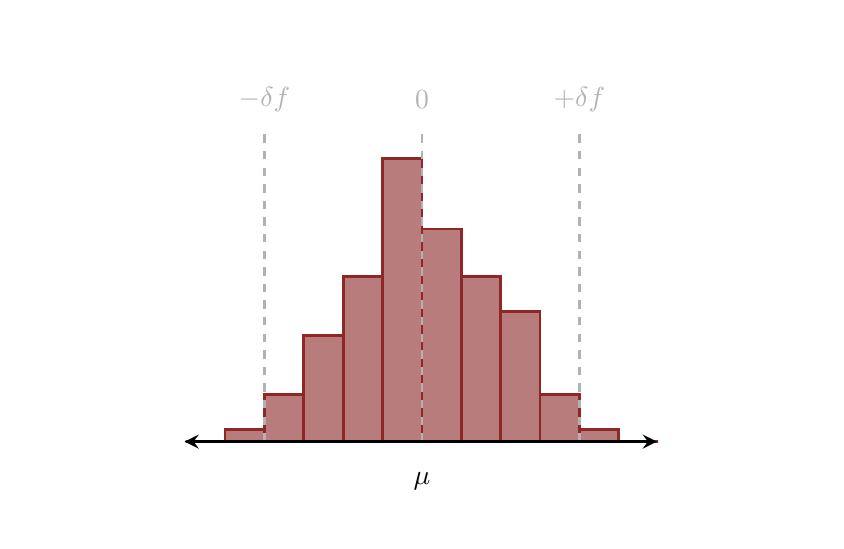
\begin{tikzpicture}[scale=1.0]

  \begin{scope}[shift={(0, 0)}]
    \draw[white] (-5, -3) rectangle (5, 3.25);

    \foreach \c/\b in {0.000/-3.000, 1.000/-2.500, 4.000/-2.000, 
                       9.000/-1.500, 14.000/-1.000, 24.000/-0.500, 
                       18.000/0.000, 14.000/0.500, 11.000/1.000, 
                       4.000/1.500, 1.000/2.000, 0.000/2.500} {
      \filldraw[fill=mid, draw=dark, line width=1] (\b, -2) rectangle ({\b + 0.5}, {0.15 * \c - 2});
    }

    \draw[gray70, dashed, line width=1] (+ 2, -2) -- (+ 2, 2);
    \draw[gray70, dashed, line width=1] (0, -2) -- (0, 2);
    \draw[gray70, dashed, line width=1] (- 2, -2) -- (- 2, 2);
    \node[gray70] at (0, 2.35) { $0$ };
    \node[gray70] at (0 - 2, 2.35) { $-\delta f$ };
    \node[gray70] at (0 + 2, 2.35) { $+\delta f$ };

    \draw [<->, >=stealth, line width=1.25] (-3.015, -2.00) -- +(6, 0);
    \node at (0, -2.5) { $\mu$ };
  \end{scope}
  
\end{tikzpicture}

\end{document}  